%%%%%%%%%%%%%%%%%%%%%%%%%%%%%%%%%%%%%%%%%
% The Legrand Orange Book
% LaTeX Template
% Version 1.4 (12/4/14)
%
% This template has been downloaded from:
% http://www.LaTeXTemplates.com
%
% Original author:
% Mathias Legrand (legrand.mathias@gmail.com)
%
% License:
% CC BY-NC-SA 3.0 (http://creativecommons.org/licenses/by-nc-sa/3.0/)
%
% Compiling this template:
% This template uses biber for its bibliography and makeindex for its index.
% When you first open the template, compile it from the command line with the 
% commands below to make sure your LaTeX distribution is configured correctly:
%
% 1) pdflatex main
% 2) makeindex main.idx -s StyleInd.ist
% 3) biber main
% 4) pdflatex main x 2
%
% After this, when you wish to update the bibliography/index use the appropriate
% command above and make sure to compile with pdflatex several times 
% afterwards to propagate your changes to the document.
%
% This template also uses a number of packages which may need to be
% updated to the newest versions for the template to compile. It is strongly
% recommended you update your LaTeX distribution if you have any
% compilation errors.
%
% Important note:
% Chapter heading images should have a 2:1 width:height ratio,
% e.g. 920px width and 460px height.
%
%%%%%%%%%%%%%%%%%%%%%%%%%%%%%%%%%%%%%%%%%

%----------------------------------------------------------------------------------------
%	PACKAGES AND OTHER DOCUMENT CONFIGURATIONS
%----------------------------------------------------------------------------------------

\documentclass[11pt,fleqn]{book} % Default font size and left-justified equations

\usepackage[top=3cm,bottom=3cm,left=3.2cm,right=3.2cm,headsep=10pt,a4paper]{geometry} % Page margins
\usepackage{tabularx}
\usepackage{tabulary}
\usepackage{booktabs}

\usepackage{xcolor} % Required for specifying colors by name
\definecolor{ocre}{RGB}{243,102,25} % Define the orange color used for highlighting throughout the book

% Font Settings
\usepackage{avant} % Use the Avantgarde font for headings
%\usepackage{times} % Use the Times font for headings
\usepackage{mathptmx} % Use the Adobe Times Roman as the default text font together with math symbols from the Sym­bol, Chancery and Com­puter Modern fonts

\usepackage{microtype} % Slightly tweak font spacing for aesthetics
\usepackage[utf8]{inputenc} % Required for including letters with accents
\usepackage[T1]{fontenc} % Use 8-bit encoding that has 256 glyphs

% Bibliography
\usepackage[autostyle]{csquotes}
\usepackage[
        style=numeric-comp,
        sorting=none, 
        sortcites=true,
        sortlocale=en_GB,
        autopunct=true,
        babel=hyphen,
        hyperref=true,
        url=true, 
        abbreviate=false,
        backref=true,
        arxiv=abs,
        backend=biber]{biblatex}
\addbibresource{BroadwickManual.bib} % BibTeX bibliography file
\defbibheading{bibempty}{}






% Index
\usepackage{calc} % For simpler calculation - used for spacing the index letter headings correctly
\usepackage{makeidx} % Required to make an index
\makeindex % Tells LaTeX to create the files required for indexing

% code listing
\usepackage{listings}
\usepackage{color}


%----------------------------------------------------------------------------------------

%----------------------------------------------------------------------------------------
%	VARIOUS REQUIRED PACKAGES
%----------------------------------------------------------------------------------------

\usepackage{titlesec} % Allows customization of titles

\usepackage{graphicx} % Required for including pictures
\graphicspath{{img/}} % Specifies the directory where pictures are stored

\usepackage{lipsum} % Inserts dummy text

\usepackage{tikz} % Required for drawing custom shapes

\usepackage[english]{babel} % English language/hyphenation

\usepackage{enumitem} % Customize lists
\setlist{nolistsep} % Reduce spacing between bullet points and numbered lists

\usepackage{booktabs} % Required for nicer horizontal rules in tables

\usepackage{eso-pic} % Required for specifying an image background in the title page

%----------------------------------------------------------------------------------------
%	MAIN TABLE OF CONTENTS
%----------------------------------------------------------------------------------------

\usepackage{titletoc} % Required for manipulating the table of contents

\contentsmargin{0cm} % Removes the default margin
% Chapter text styling
\titlecontents{chapter}[1.25cm] % Indentation
{\addvspace{15pt}\large\sffamily\bfseries} % Spacing and font options for chapters
{\color{ocre!60}\contentslabel[\Large\thecontentslabel]{1.25cm}\color{ocre}} % Chapter number
{}  
{\color{ocre!60}\normalsize\sffamily\bfseries\;\titlerule*[.5pc]{.}\;\thecontentspage} % Page number
% Section text styling
\titlecontents{section}[1.25cm] % Indentation
{\addvspace{5pt}\sffamily\bfseries} % Spacing and font options for sections
{\contentslabel[\thecontentslabel]{1.25cm}} % Section number
{}
{\sffamily\hfill\color{black}\thecontentspage} % Page number
[]
% Subsection text styling
\titlecontents{subsection}[1.25cm] % Indentation
{\addvspace{1pt}\sffamily\small} % Spacing and font options for subsections
{\contentslabel[\thecontentslabel]{1.25cm}} % Subsection number
{}
{\sffamily\;\titlerule*[.5pc]{.}\;\thecontentspage} % Page number
[] 

%----------------------------------------------------------------------------------------
%	MINI TABLE OF CONTENTS IN CHAPTER HEADS
%----------------------------------------------------------------------------------------

% Section text styling
\titlecontents{lsection}[0em] % Indendating
{\footnotesize\sffamily} % Font settings
{}
{}
{}

% Subsection text styling
\titlecontents{lsubsection}[.5em] % Indentation
{\normalfont\footnotesize\sffamily} % Font settings
{}
{}
{}
 
%----------------------------------------------------------------------------------------
%	PAGE HEADERS
%----------------------------------------------------------------------------------------

\usepackage{fancyhdr} % Required for header and footer configuration

\pagestyle{fancy}
\renewcommand{\chaptermark}[1]{\markboth{\sffamily\normalsize\bfseries\chaptername\ \thechapter.\ #1}{}} % Chapter text font settings
\renewcommand{\sectionmark}[1]{\markright{\sffamily\normalsize\thesection\hspace{5pt}#1}{}} % Section text font settings
\fancyhf{} \fancyhead[LE,RO]{\sffamily\normalsize\thepage} % Font setting for the page number in the header
\fancyhead[LO]{\rightmark} % Print the nearest section name on the left side of odd pages
\fancyhead[RE]{\leftmark} % Print the current chapter name on the right side of even pages
\renewcommand{\headrulewidth}{0.5pt} % Width of the rule under the header
\addtolength{\headheight}{2.5pt} % Increase the spacing around the header slightly
\renewcommand{\footrulewidth}{0pt} % Removes the rule in the footer
\fancypagestyle{plain}{\fancyhead{}\renewcommand{\headrulewidth}{0pt}} % Style for when a plain pagestyle is specified

% Removes the header from odd empty pages at the end of chapters
\makeatletter
\renewcommand{\cleardoublepage}{
\clearpage\ifodd\c@page\else
\hbox{}
\vspace*{\fill}
\thispagestyle{empty}
\newpage
\fi}


%----------------------------------------------------------------------------------------
%	CODE SNIPPETS
%----------------------------------------------------------------------------------------

\definecolor{dkgreen}{rgb}{0,0.6,0}
\definecolor{gray}{rgb}{0.5,0.5,0.5}
\definecolor{mauve}{rgb}{0.58,0,0.82}

\lstset{frame=tb,
  language=Java,
  aboveskip=3mm,
  belowskip=3mm,
  showstringspaces=false,
  columns=flexible,
  basicstyle={\small\ttfamily},
  numbers=none,
  numberstyle=\tiny\color{gray},
  keywordstyle=\color{blue},
  commentstyle=\color{dkgreen},
  stringstyle=\color{mauve},
  breaklines=true,
  breakatwhitespace=true,
  tabsize=3
}

%----------------------------------------------------------------------------------------
%	THEOREM STYLES
%----------------------------------------------------------------------------------------

\usepackage{amsmath,amsfonts,amssymb,amsthm} % For math equations, theorems, symbols, etc

\newcommand{\intoo}[2]{\mathopen{]}#1\,;#2\mathclose{[}}
\newcommand{\ud}{\mathop{\mathrm{{}d}}\mathopen{}}
\newcommand{\intff}[2]{\mathopen{[}#1\,;#2\mathclose{]}}
\newtheorem{notation}{Notation}[chapter]

%%%%%%%%%%%%%%%%%%%%%%%%%%%%%%%%%%%%%%%%%%%%%%%%%%%%%%%%%%%%%%%%%%%%%%%%%%%
%%%%%%%%%%%%%%%%%%%% dedicated to boxed/framed environements %%%%%%%%%%%%%%
%%%%%%%%%%%%%%%%%%%%%%%%%%%%%%%%%%%%%%%%%%%%%%%%%%%%%%%%%%%%%%%%%%%%%%%%%%%
\newtheoremstyle{ocrenumbox}% % Theorem style name
{0pt}% Space above
{0pt}% Space below
{\normalfont}% % Body font
{}% Indent amount
{\small\bf\sffamily\color{ocre}}% % Theorem head font
{\;}% Punctuation after theorem head
{0.25em}% Space after theorem head
{\small\sffamily\color{ocre}\thmname{#1}\nobreakspace\thmnumber{\@ifnotempty{#1}{}\@upn{#2}}% Theorem text (e.g. Theorem 2.1)
\thmnote{\nobreakspace\the\thm@notefont\sffamily\bfseries\color{black}---\nobreakspace#3.}} % Optional theorem note
\renewcommand{\qedsymbol}{$\blacksquare$}% Optional qed square

\newtheoremstyle{blacknumex}% Theorem style name
{5pt}% Space above
{5pt}% Space below
{\normalfont}% Body font
{} % Indent amount
{\small\bf\sffamily}% Theorem head font
{\;}% Punctuation after theorem head
{0.25em}% Space after theorem head
{\small\sffamily{\tiny\ensuremath{\blacksquare}}\nobreakspace\thmname{#1}\nobreakspace\thmnumber{\@ifnotempty{#1}{}\@upn{#2}}% Theorem text (e.g. Theorem 2.1)
\thmnote{\nobreakspace\the\thm@notefont\sffamily\bfseries---\nobreakspace#3.}}% Optional theorem note

\newtheoremstyle{blacknumbox} % Theorem style name
{0pt}% Space above
{0pt}% Space below
{\normalfont}% Body font
{}% Indent amount
{\small\bf\sffamily}% Theorem head font
{\;}% Punctuation after theorem head
{0.25em}% Space after theorem head
{\small\sffamily\thmname{#1}\nobreakspace\thmnumber{\@ifnotempty{#1}{}\@upn{#2}}% Theorem text (e.g. Theorem 2.1)
\thmnote{\nobreakspace\the\thm@notefont\sffamily\bfseries---\nobreakspace#3.}}% Optional theorem note

%%%%%%%%%%%%%%%%%%%%%%%%%%%%%%%%%%%%%%%%%%%%%%%%%%%%%%%%%%%%%%%%%%%%%%%%%%%
%%%%%%%%%%%%% dedicated to non-boxed/non-framed environements %%%%%%%%%%%%%
%%%%%%%%%%%%%%%%%%%%%%%%%%%%%%%%%%%%%%%%%%%%%%%%%%%%%%%%%%%%%%%%%%%%%%%%%%%
\newtheoremstyle{ocrenum}% % Theorem style name
{5pt}% Space above
{5pt}% Space below
{\normalfont}% % Body font
{}% Indent amount
{\small\bf\sffamily\color{ocre}}% % Theorem head font
{\;}% Punctuation after theorem head
{0.25em}% Space after theorem head
{\small\sffamily\color{ocre}\thmname{#1}\nobreakspace\thmnumber{\@ifnotempty{#1}{}\@upn{#2}}% Theorem text (e.g. Theorem 2.1)
\thmnote{\nobreakspace\the\thm@notefont\sffamily\bfseries\color{black}---\nobreakspace#3.}} % Optional theorem note
\renewcommand{\qedsymbol}{$\blacksquare$}% Optional qed square
\makeatother

% Defines the theorem text style for each type of theorem to one of the three styles above
\newcounter{dummy} 
\numberwithin{dummy}{section}
\theoremstyle{ocrenumbox}
\newtheorem{theoremeT}[dummy]{Theorem}
\newtheorem{problem}{Problem}[chapter]
\newtheorem{exerciseT}{Exercise}[chapter]
\theoremstyle{blacknumex}
\newtheorem{exampleT}{Example}[chapter]
\theoremstyle{blacknumbox}
\newtheorem{vocabulary}{Vocabulary}[chapter]
\newtheorem{definitionT}{Definition}[section]
\newtheorem{corollaryT}[dummy]{Corollary}
\theoremstyle{ocrenum}
\newtheorem{proposition}[dummy]{Proposition}

%----------------------------------------------------------------------------------------
%	DEFINITION OF COLORED BOXES
%----------------------------------------------------------------------------------------

\RequirePackage[framemethod=default]{mdframed} % Required for creating the theorem, definition, exercise and corollary boxes

% Theorem box
\newmdenv[skipabove=7pt,
skipbelow=7pt,
backgroundcolor=black!5,
linecolor=ocre,
innerleftmargin=5pt,
innerrightmargin=5pt,
innertopmargin=5pt,
leftmargin=0cm,
rightmargin=0cm,
innerbottommargin=5pt]{tBox}

% Exercise box	  
\newmdenv[skipabove=7pt,
skipbelow=7pt,
rightline=false,
leftline=true,
topline=false,
bottomline=false,
backgroundcolor=ocre!10,
linecolor=ocre,
innerleftmargin=5pt,
innerrightmargin=5pt,
innertopmargin=5pt,
innerbottommargin=5pt,
leftmargin=0cm,
rightmargin=0cm,
linewidth=4pt]{eBox}	

% Definition box
\newmdenv[skipabove=7pt,
skipbelow=7pt,
rightline=false,
leftline=true,
topline=false,
bottomline=false,
linecolor=ocre,
innerleftmargin=5pt,
innerrightmargin=5pt,
innertopmargin=0pt,
leftmargin=0cm,
rightmargin=0cm,
linewidth=4pt,
innerbottommargin=0pt]{dBox}	

% Corollary box
\newmdenv[skipabove=7pt,
skipbelow=7pt,
rightline=false,
leftline=true,
topline=false,
bottomline=false,
linecolor=gray,
backgroundcolor=black!5,
innerleftmargin=5pt,
innerrightmargin=5pt,
innertopmargin=5pt,
leftmargin=0cm,
rightmargin=0cm,
linewidth=4pt,
innerbottommargin=5pt]{cBox}

% Code box
\newmdenv[skipabove=7pt,
skipbelow=7pt,
rightline=false,
leftline=true,
topline=false,
bottomline=false,
linecolor=gray,
backgroundcolor=black!5,
innerleftmargin=5pt,
innerrightmargin=5pt,
innertopmargin=5pt,
leftmargin=0cm,
rightmargin=0cm,
linewidth=4pt,
innerbottommargin=5pt]{sBox}
% Creates an environment for each type of theorem and assigns it a theorem text style from the "Theorem Styles" section above and a colored box from above
\newenvironment{theorem}{\begin{tBox}\begin{theoremeT}}{\end{theoremeT}\end{tBox}}
\newenvironment{exercise}{\begin{eBox}\begin{exerciseT}}{\hfill{\color{ocre}\tiny\ensuremath{\blacksquare}}\end{exerciseT}\end{eBox}}				  
\newenvironment{definition}{\begin{dBox}\begin{definitionT}}{\end{definitionT}\end{dBox}}	
\newenvironment{example}{\begin{exampleT}}{\hfill{\tiny\ensuremath{\blacksquare}}\end{exampleT}}		
\newenvironment{corollary}{\begin{cBox}\begin{corollaryT}}{\end{corollaryT}\end{cBox}}	
\newenvironment{sourcecode}{\begin{sBox}}{\end{sBox}}	

%----------------------------------------------------------------------------------------
%	REMARK ENVIRONMENT
%----------------------------------------------------------------------------------------

\newenvironment{remark}{\par\vspace{10pt}\small % Vertical white space above the remark and smaller font size
\begin{list}{}{
\leftmargin=35pt % Indentation on the left
\rightmargin=25pt}\item\ignorespaces % Indentation on the right
\makebox[-2.5pt]{\begin{tikzpicture}[overlay]
\node[draw=ocre!60,line width=1pt,circle,fill=ocre!25,font=\sffamily\bfseries,inner sep=2pt,outer sep=0pt] at (-15pt,0pt){\textcolor{ocre}{R}};\end{tikzpicture}} % Orange R in a circle
\advance\baselineskip -1pt}{\end{list}\vskip5pt} % Tighter line spacing and white space after remark

%----------------------------------------------------------------------------------------
%	SECTION NUMBERING IN THE MARGIN
%----------------------------------------------------------------------------------------

\makeatletter
\renewcommand{\@seccntformat}[1]{\llap{\textcolor{ocre}{\csname the#1\endcsname}\hspace{1em}}}                    
\renewcommand{\section}{\@startsection{section}{1}{\z@}
{-4ex \@plus -1ex \@minus -.4ex}
{1ex \@plus.2ex }
{\normalfont\large\sffamily\bfseries}}
\renewcommand{\subsection}{\@startsection {subsection}{2}{\z@}
{-3ex \@plus -0.1ex \@minus -.4ex}
{0.5ex \@plus.2ex }
{\normalfont\sffamily\bfseries}}
\renewcommand{\subsubsection}{\@startsection {subsubsection}{3}{\z@}
{-2ex \@plus -0.1ex \@minus -.2ex}
{.2ex \@plus.2ex }
{\normalfont\small\sffamily\bfseries}}                        
\renewcommand\paragraph{\@startsection{paragraph}{4}{\z@}
{-2ex \@plus-.2ex \@minus .2ex}
{.1ex}
{\normalfont\small\sffamily\bfseries}}

%----------------------------------------------------------------------------------------
%	HYPERLINKS IN THE DOCUMENTS
%----------------------------------------------------------------------------------------

% For an unclear reason, the package should be loaded now and not later
\usepackage{hyperref}
\hypersetup{hidelinks,backref=true,pagebackref=true,hyperindex=true,colorlinks=false,breaklinks=true,urlcolor= ocre,bookmarks=true,bookmarksopen=false,pdftitle={Title},pdfauthor={Author}}

%----------------------------------------------------------------------------------------
%	CHAPTER HEADINGS
%----------------------------------------------------------------------------------------

% The set-up below should be (sadly) manually adapted to the overall margin page septup controlled by the geometry package loaded in the main.tex document. It is possible to implement below the dimensions used in the goemetry package (top,bottom,left,right)... TO BE DONE

\newcommand{\thechapterimage}{}
\newcommand{\chapterimage}[1]{\renewcommand{\thechapterimage}{#1}}

% Numbered chapters with mini tableofcontents
\def\thechapter{\arabic{chapter}}
\def\@makechapterhead#1{
\thispagestyle{empty}
{\centering \normalfont\sffamily
\ifnum \c@secnumdepth >\m@ne
\if@mainmatter
\startcontents
\begin{tikzpicture}[remember picture,overlay]
\node at (current page.north west)
{\begin{tikzpicture}[remember picture,overlay]
\node[anchor=north west,inner sep=0pt] at (0,0) {\includegraphics[width=\paperwidth]{\thechapterimage}};
%%%%%%%%%%%%%%%%%%%%%%%%%%%%%%%%%%%%%%%%%%%%%%%%%%%%%%%%%%%%%%%%%%%%%%%%%%%%%%%%%%%%%
% Commenting the 3 lines below removes the small contents box in the chapter heading
\fill[color=ocre!10!white,opacity=.6] (1cm,0) rectangle (8cm,-7cm);
\node[anchor=north west] at (1.1cm,.35cm) {\parbox[t][8cm][t]{6.5cm}{\huge\bfseries\flushleft \printcontents{l}{1}{\setcounter{tocdepth}{2}}}};
\draw[anchor=west] (5cm,-9cm) node [rounded corners=20pt,fill=ocre!10!white,text opacity=1,draw=ocre,draw opacity=1,line width=1.5pt,fill opacity=.6,inner sep=12pt]{\huge\sffamily\bfseries\textcolor{black}{\thechapter. #1\strut\makebox[22cm]{}}};
%%%%%%%%%%%%%%%%%%%%%%%%%%%%%%%%%%%%%%%%%%%%%%%%%%%%%%%%%%%%%%%%%%%%%%%%%%%%%%%%%%%%%
\end{tikzpicture}};
\end{tikzpicture}}
\par\vspace*{230\p@}
\fi
\fi}

% Unnumbered chapters without mini tableofcontents (could be added though) 
\def\@makeschapterhead#1{
\thispagestyle{empty}
{\centering \normalfont\sffamily
\ifnum \c@secnumdepth >\m@ne
\if@mainmatter
\begin{tikzpicture}[remember picture,overlay]
\node at (current page.north west)
{\begin{tikzpicture}[remember picture,overlay]
\node[anchor=north west,inner sep=0pt] at (0,0) {\includegraphics[width=\paperwidth]{\thechapterimage}};
\draw[anchor=west] (5cm,-9cm) node [rounded corners=20pt,fill=ocre!10!white,fill opacity=.6,inner sep=12pt,text opacity=1,draw=ocre,draw opacity=1,line width=1.5pt]{\huge\sffamily\bfseries\textcolor{black}{#1\strut\makebox[22cm]{}}};
\end{tikzpicture}};
\end{tikzpicture}}
\par\vspace*{230\p@}
\fi
\fi
}
\makeatother
 % Insert the commands.tex file which contains the majority of the structure behind the template

\begin{document}

%----------------------------------------------------------------------------------------
%	TITLE PAGE
%----------------------------------------------------------------------------------------

\begingroup
\thispagestyle{empty}
\AddToShipoutPicture*{\put(6,5){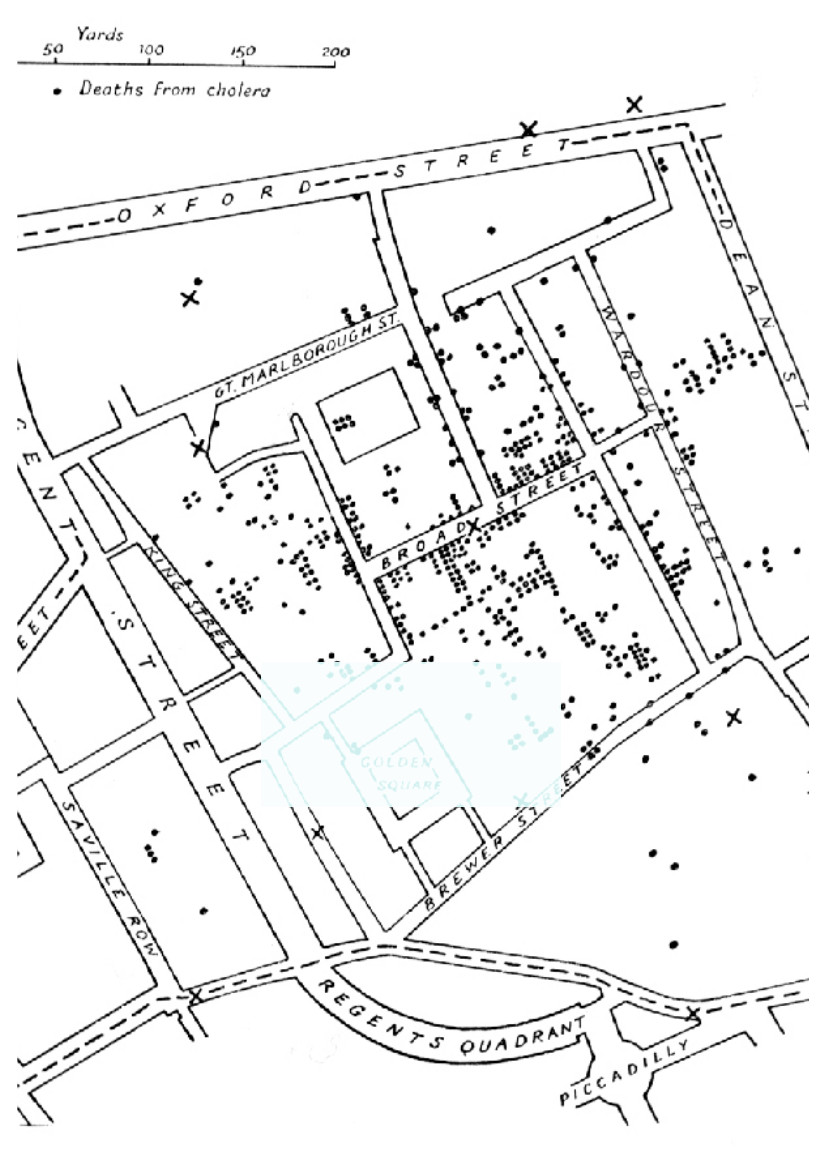
\includegraphics[scale=1]{background.jpg}}} % Image background
\centering
\vspace*{13cm}
\par\normalfont\fontsize{35}{35}\sffamily\selectfont
Broadwick\par % Book title
\vspace*{1cm}
{\Huge A Users Guide}\par % Author name
\endgroup

%----------------------------------------------------------------------------------------
%	COPYRIGHT PAGE
%----------------------------------------------------------------------------------------

\newpage
%~\vfill
\thispagestyle{empty}

\begin{center}
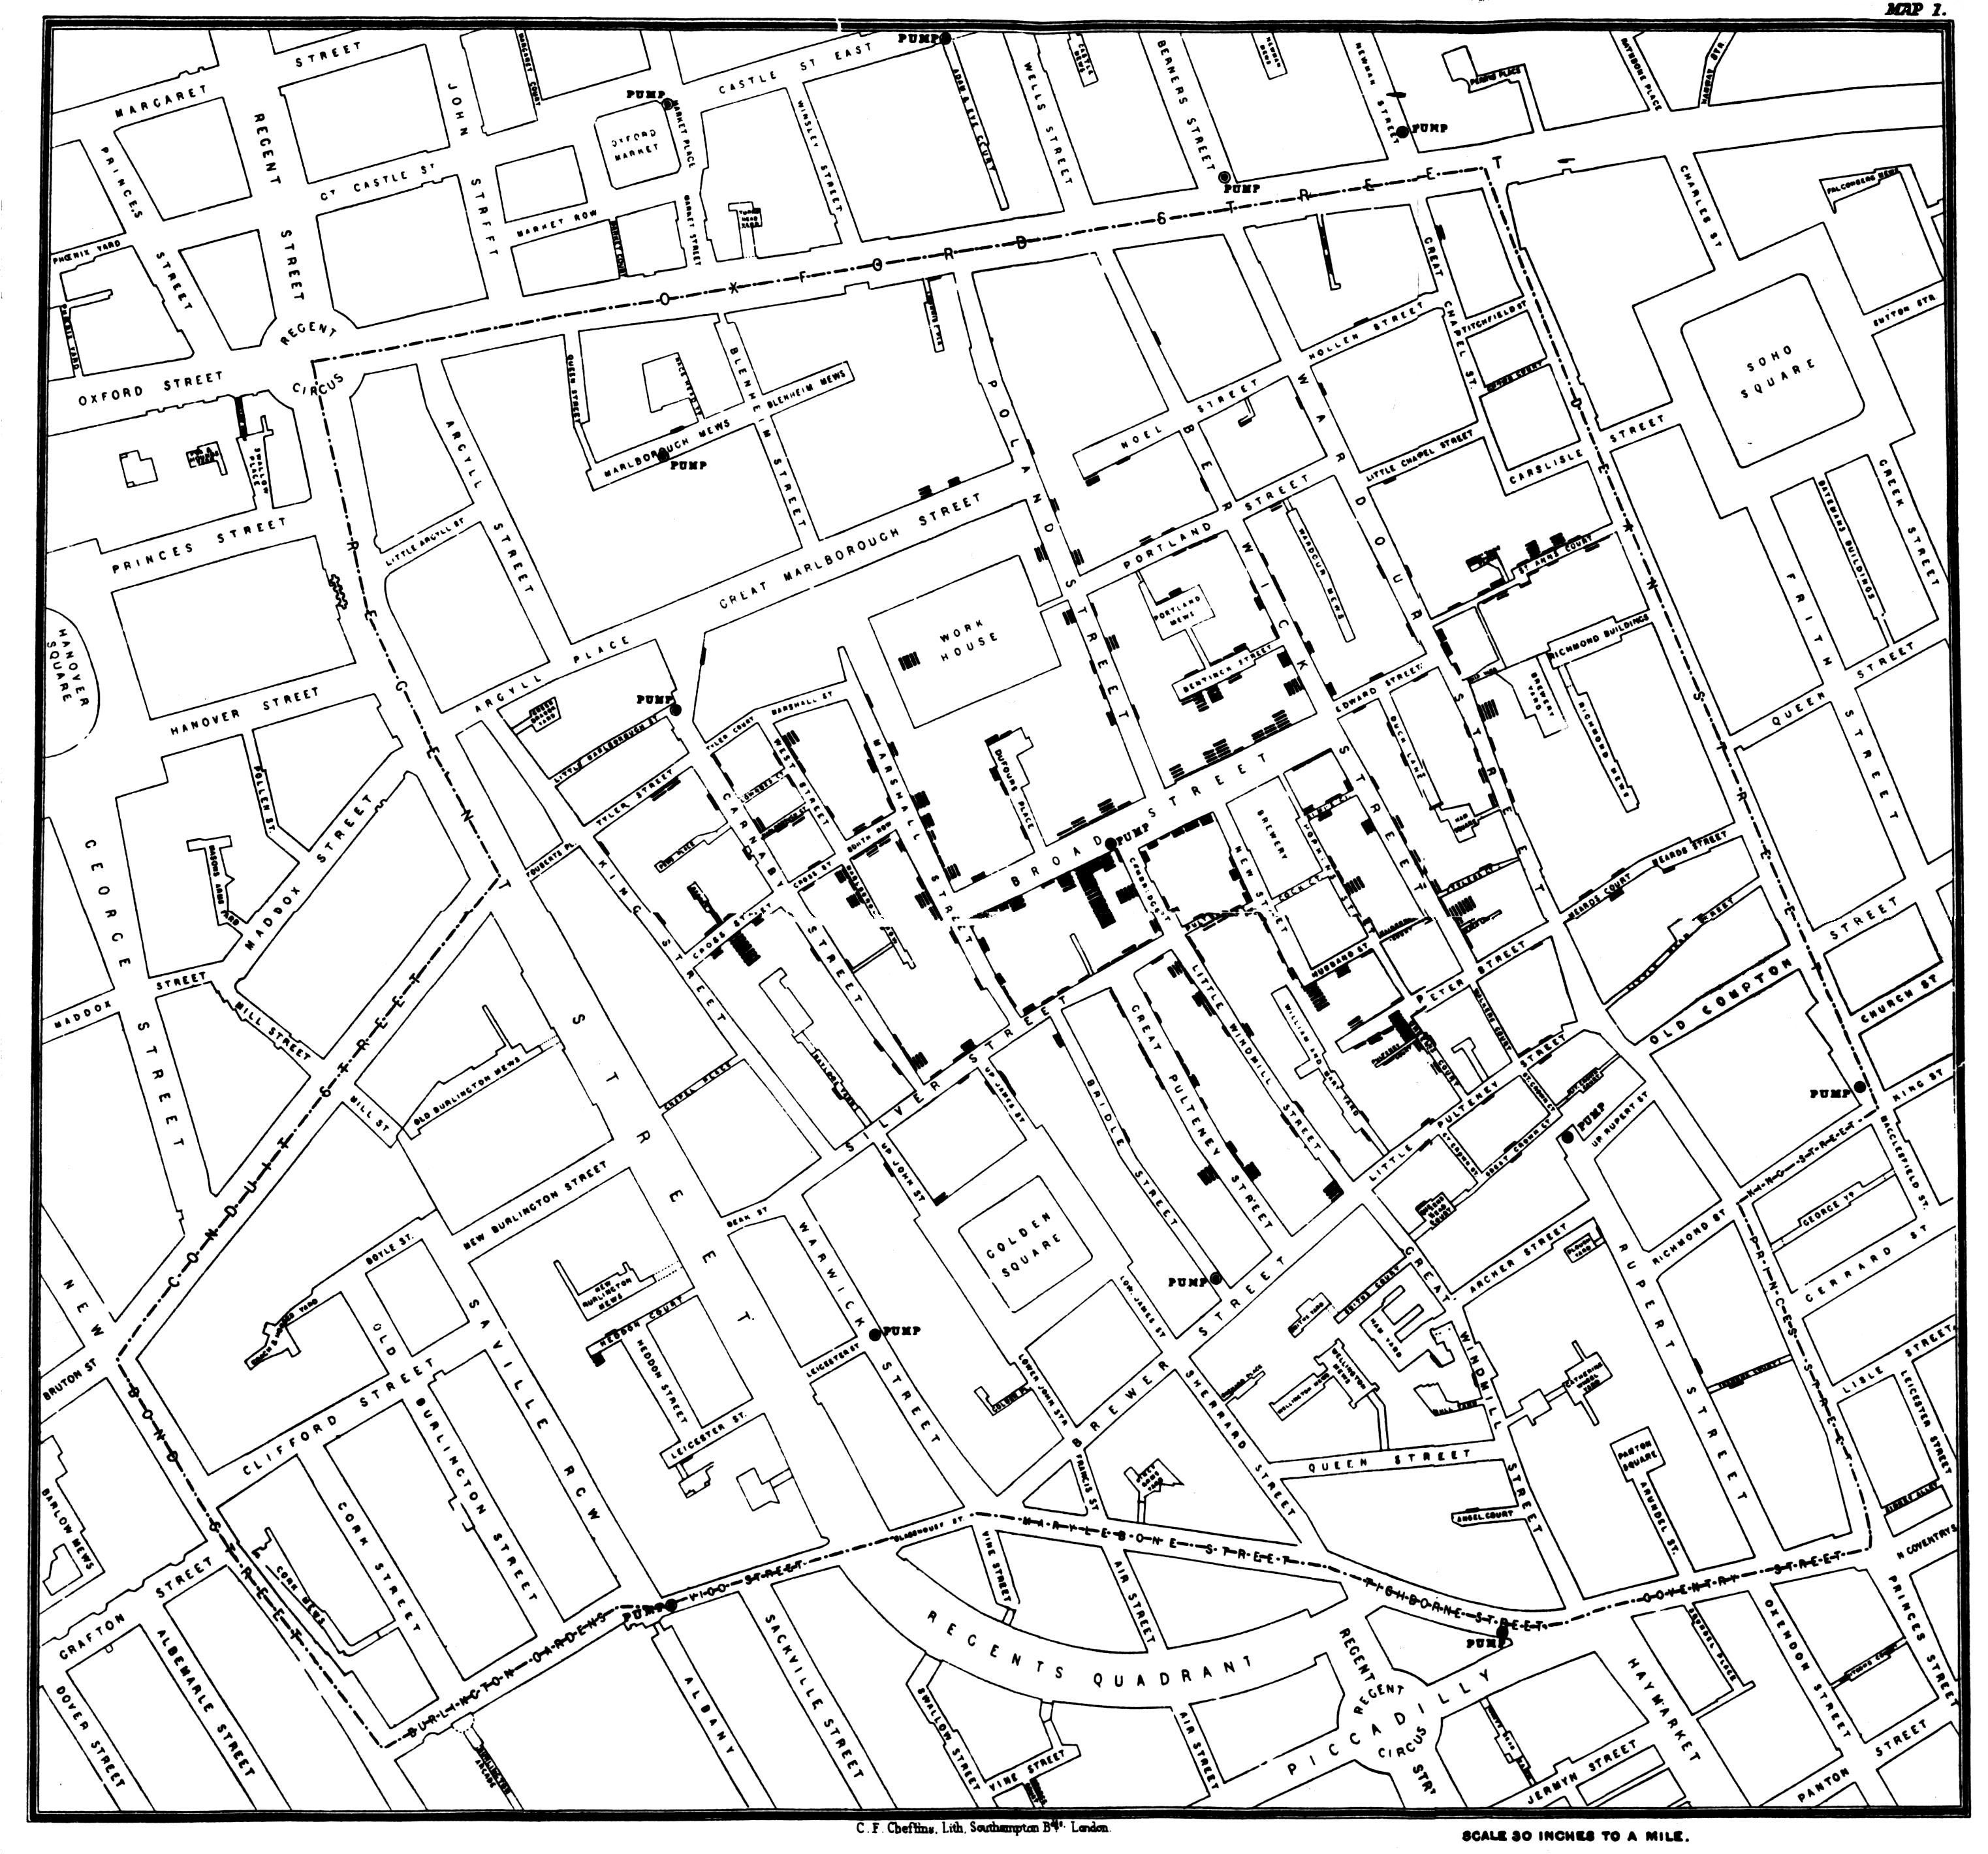
\includegraphics[scale=0.1]{Snow-cholera-map.jpg}
\end{center}

Published by C.F. Cheffins, Lith, Southhampton Buildings, London, England, 1854 in Snow, John. On the Mode of Communication of Cholera, 2nd Ed, John Churchill, New Burlington Street, London, England, 1855.
This image was originally from \emph{http://en.wikipedia.org/wiki/File:Snow-cholera-map-1.jpg}

\textbf{Cover Picture}

A variant of the original map drawn by Dr. John Snow (1813-1858), a British physician who is one of the founders of medical epidemiology, showing cases of cholera in the London epidemics of 1854, clustered around the locations of water pumps.

This image is in the public domain because its copyright has expired. This applies to Australia, the European Union and those countries with a copyright term of life of the author plus 70 years.

The figures used in the chapter headings are cropped images from \url{unsplash.com} and are licensed under Creative Commons Zero license.

~\vfill

\noindent Copyright \copyright\ 2013 University of Glasgow\\ % Copyright notice

%\noindent \textsc{Published by Publisher}\\ % Publisher

\noindent \textsc{http://epicscotland.github.io/Broadwick/}\\ % URL

\noindent Licensed under the Apache License, Version 2.0 (the "License"); you may not use this file except in compliance with the License.  You may obtain a copy of the License at \url{http://www.apache.org/licenses/LICENSE-2.0}. Unless required by applicable law or agreed to in writing, software distributed under the License is distributed on an "AS IS" BASIS, WITHOUT WARRANTIES OR CONDITIONS OF ANY KIND, either express or implied.  See the License for the specific language governing permissions and limitations under the License.\\ % License information

\noindent \textit{First printing, March 2013} % Printing/edition date

%----------------------------------------------------------------------------------------
%	TABLE OF CONTENTS
%----------------------------------------------------------------------------------------

\chapterimage{chapter_head_toc.jpg} % Table of contents heading image

\pagestyle{empty} % No headers

\tableofcontents % Print the table of contents itself

\cleardoublepage % Forces the first chapter to start on an odd page so it's on the right

\pagestyle{fancy} % Print headers again

%----------------------------------------------------------------------------------------
%	CHAPTER 1
%----------------------------------------------------------------------------------------

\chapterimage{chapter_head_2.jpg} % Chapter heading image
\chapter{Introduction}

In the event of an outbreak it is important to have modelling tools in place to estimate the likely origin, speed of spread, and size, and to be able to predict the impact of intervention measures.  However, different diseases in different animal populations require somewhat different approaches due to the detection, transmission and recovery (or not) characteristics of hosts infected with the pathogen, and the contact patterns between susceptible hosts (whether of the same species or not).  Consequently specific models developed for one disease system are unlikely to be entirely suitable for another.  

Broadwick is a framework for developing sophisticated epidemiological based mathematical models, and consists of several Java libraries and bespoke packages.  The components of Broadwick are written in such a way that a scientist may combine them in order to rapidly prototype a model for a new specific scenario.

\begin{itemize}
\item Supports single (e.g. within herd) or structured populations (e.g. multi-species or locations)
\item Inclusion of movement over network data (e.g. Cattle movement Tracing System) 
\item Stochastic Individual Based simulations (including fast approximate options) 
\item Approximate Bayesian Computation inference for estimating model parameters from data via simulations
\item Markov Chain Monte Carlo inference for estimating model parameters from data
\end{itemize}

\section{License}\index{License}

Broadwick is released under the Apache 2 license.

%\section{Notations}\index{Notations}
%
%\begin{notation}
%Given an open subset $G$ of $\mathbb{R}^n$, the set of functions $\varphi$ are:
%\begin{enumerate}
%\item Bounded support $G$;
%\item Infinitely differentiable;
%\end{enumerate}
%a vector space is denoted by $\mathcal{D}(G)$. 
%\end{notation}



\chapterimage{chapter_head_3.jpg} % Chapter heading image
\chapter{Installation}

A compiled Broadwick jar is available from the EPIC Scotland website that can be added to your project. Broadwick uses maven as its build tool and so this manual is rather maven focused. You can use Broadwick with other tools or import it into your IDE settings though this is outside the scope of this manual.

\section{Installing the Distribution Jar}
If you plan on downloading the distribution jar file you should place it under 
\begin{sourcecode}
\${HOME}/.m2/repository/broadwick/broadwick/1.2
\end{sourcecode}

\section{Installing From Source}
To download the Broadwick sources
\begin{enumerate}
\item Create a directory for broad wick and ‘cd’ into that directory
\item Copy the broadwick sources.
      \begin{sourcecode}
      git clone https://github.com/EPICScotland/Broadwick .
      \end{sourcecode}
      (this may take a while as there are release snapshots that are also on the site)
\item Build the jar library.
\begin{sourcecode}
man package install; cd archetype; man install
\end{sourcecode}

You should see output similar to
\begin{sourcecode}
INFO --- maven-compiler-plugin:3.1:compile (default-compile) @ broadwick ---
INFO Changes detected - recompiling the module!
INFO Compiling 157 source files to /XXXX/XXXX/XXXX/EPICScotland/Broadwick/target/classes
WARNING bootstrap class path not set in conjunction with -source 1.7
WARNING No processor claimed any of these annotations: javax.xml.bind.annotation.XmlAccessorType,javax.xml.bind.annotation.XmlAttribute,lombok.Synchronized,lombok.Setter,lombok.Getter,lombok.EqualsAndHashCode,javax.xml.bind.annotation.XmlRootElement,javax.xml.bind.annotation.XmlSeeAlso,lombok.extern.slf4j.Slf4j,javax.xml.bind.annotation.XmlType,javax.xml.bind.annotation.XmlElements,javax.xml.bind.annotation.XmlRegistry,lombok.Data,lombok.ToString,javax.xml.bind.annotation.XmlElement
\end{sourcecode}

      This will install the broadwick jar and the archetype under .m2/repository/broadwick/broadwick/1.2

\end{enumerate}

Now you can create a new project using this archetype:
\begin{sourcecode}
mvn3 archetype:generate -DarchetypeGroupId=broadwick -DarchetypeArtifactId=broadwick- archetype -DarchetypeVersion=1.2 -DgroupId=<unique id for your project> -DartifactId=<your project name> -Dversion=0.1 -Dpackage=<your package> 
\end{sourcecode}




\section{Ubuntu}

The version of Java on Ubuntu 15.04 (other versions are also possibley affected) causes the following error when compiling Broadwick due to the jaxb plugin which is used to generate java sources.

\begin{sourcecode}
WARNING: Error injecting: org.jvnet.mjiip.v\_2.XJC2Mojo
java.lang.NoClassDefFoundError: com/sun/xml/bind/api/ErrorListener \
	at java.lang.ClassLoader.defineClass1(Native Method)  \
	at java.lang.ClassLoader.defineClass(ClassLoader.java:800) \
	at java.security.SecureClassLoader.defineClass(SecureClassLo
\end{sourcecode}

We reccommend using the version of Java from Oracle. The following steps show how to download and install Java on Ubuntu (it is possible to revert back to Ubuntu's version afterwards).
\begin{enumerate}

\item Download the 32-bit or 64-bit Linux "compressed binary file" - it has a ".tar.gz" file extension.
\item Uncompress it
\begin{sourcecode}
		 tar -xvf jdk-8u71-linux-x64.tar.gz (32-bit)
\end{sourcecode}

    		The JDK 8 package is extracted into ./jdk1.8.0\_71 directory. N.B.: Check carefully this folder name since Oracle seem to change this occasionally with each update.

\item Move the JDK 8 directory to /usr/lib

\begin{sourcecode}
    		sudo mkdir -p /usr/lib/jvm
    		sudo mv ./jdk1.8.0\_71 /usr/lib/jvm/
\end{sourcecode}

\item Now run

\begin{sourcecode}
    		sudo update-alternatives --install "/usr/bin/java" "java" "/usr/lib/jvm/jdk1.8.0\_71/bin/java" 1
    		sudo update-alternatives --install "/usr/bin/javac" "javac" "/usr/lib/jvm/jdk1.8.0\_71/bin/javac" 1
    		sudo update-alternatives --install "/usr/bin/javaws" "javaws" "/usr/lib/jvm/jdk1.8.0\_71/bin/javaws" 1
\end{sourcecode}

    	This will assign Oracle JDK a priority of 1, which means that installing other JDKs will replace it as the default. Be sure to use a higher priority if you want Oracle JDK to remain the default.

\item Correct the file ownership and the permissions of the executables:

\begin{sourcecode}
   		sudo chmod a+x /usr/bin/java
    		sudo chmod a+x /usr/bin/javac
    		sudo chmod a+x /usr/bin/javaws
    		sudo chown -R root:root /usr/lib/jvm/jdk1.8.0\_71
\end{sourcecode}

     	N.B.: Remember - Java JDK has many more executables that you can similarly install as above. java, javac, javaws are probably the most frequently required. This answer lists the other executables available.

\item Run

\begin{sourcecode}
    		sudo update-alternatives --config java
\end{sourcecode}

    You will see output similar to the one below - choose the number of jdk1.8.0\_71

\begin{sourcecode}
    sudo update-alternatives --config java
\end{sourcecode}
    There are 3 choices for the alternative java (providing /usr/bin/java).

\begin{sourcecode}
      Selection    Path                                            Priority   Status
    ------------------------------------------------------------ \
    *  0            /usr/lib/jvm/java-7-openjdk-amd64/jre/bin/java   1071      auto mode \
      1            /usr/lib/jvm/java-7-openjdk-amd64/jre/bin/java   1071      manual mode
      2            /usr/lib/jvm/jdk1.8.0\_71/bin/java                   1         manual mode
\end{sourcecode}

\end{enumerate}
 



\chapterimage{chapter_head_4.jpg} % Chapter heading image
\chapter{Using Broadwick}

\section{Creating a New Project}\index{Creating a New Project}

Broadwick contains a set of packages that can be used as required. The framework is designed to be flexible and does not place any requirement on the user on how to use the framework. It is possible to use the classes and packages of Broadwick without using the powerful framework, creating your own main() method and taking responsibility for reading data files and configuration items though this is not the recommended way of using Broadwick.

\subsection{Using The Command Line}\index{Using The Command Line}

The Broadwick distribution contains a maven archetype for generating a skeleton project that contains all the configuration files, source code etc that is required to start a project based upon Broadwick. It uses apache maven as it’s build tool. To generate a skeleton using this archetype on the command line (assuming that the broadwick-archetype jar is in your local repository) 

\begin{sourcecode}
mvn3 archetype:generate -DarchetypeGroupId=broadwick -DarchetypeArtifactId=broadwick-archetype \
-DarchetypeVersion=1.1 -DgroupId=broadwick.proj -DartifactId=StochasticSir -Dversion=0.1 \
-Dpackage=broadwick.stochasticsir
\end{sourcecode}

The groupId (maven uses the group id to uniquely identify your project), artifactId (is the name of your generated jar file without a version), version (the version number for your generated project) and the package to which the generated source will be created can be changed by modifiying the  -DgroupId, -DartifactId, -Dversion and -Dpackage arguments above.

\subsection{Using Netbeans}\index{Using Netbeans}

It is possibly easier to create a project using Netbeans (a free IDE available form Oracle, the ‘owners’ of Java). Open the Netbeans IDE and select File->New Project and choose a Maven project and “Project from Archetype” from the list of projects (see fig{proj1}).

\begin{figure}[h]
\centering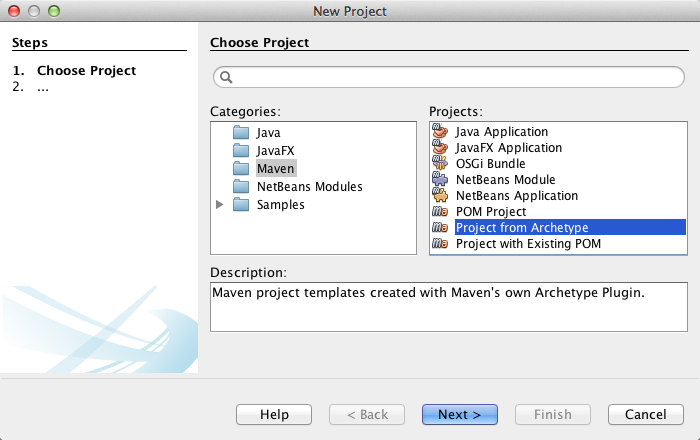
\includegraphics[width=12cm]{proj1.png}
\caption{Creating a maven based project}
\label{proj1}
\end{figure}

Click Next and choose the latest version of the broadwick-archetype from the ``Known Archetypes” (see fig \ref{proj2}). The version of the broadwick archetype corresponds to the version of Broadwick.

\begin{figure}[h!]
\centering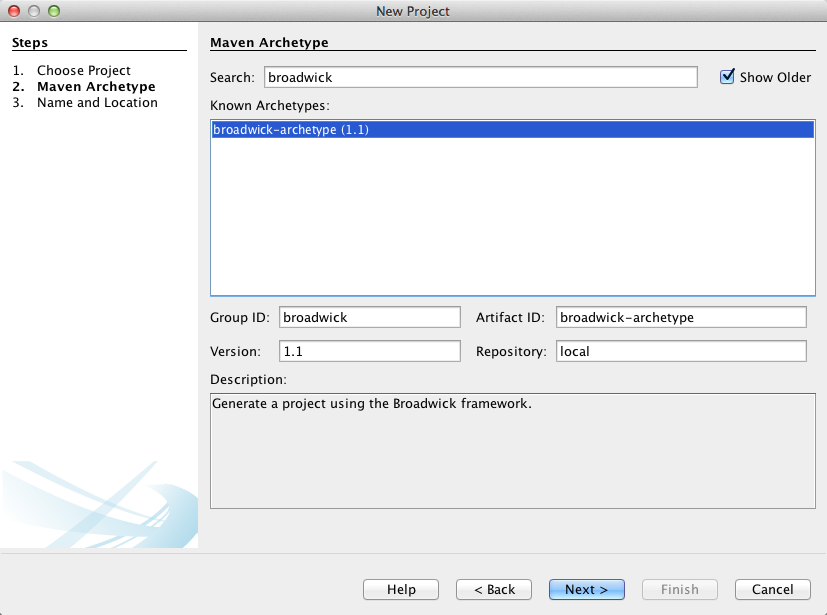
\includegraphics[width=12cm]{proj2.png}
\caption{Using the Broadwick archetype to create a skeleton project.}
\label{proj2}
\end{figure}

The projects details can be specified on the next screen (fig \ref{proj3}).

\begin{figure}[h!]
\centering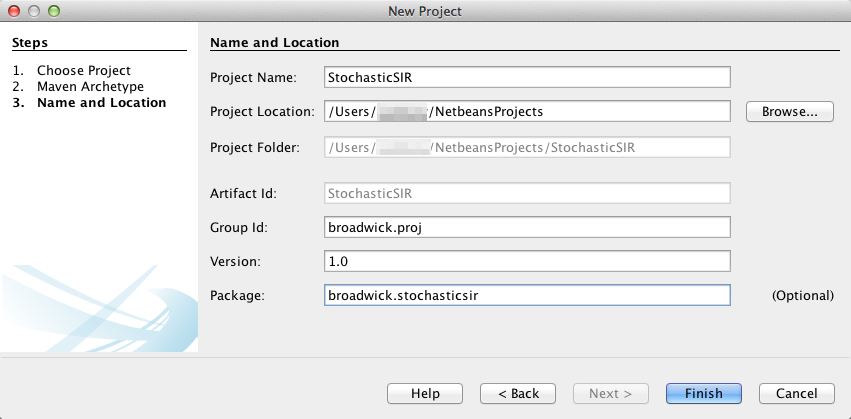
\includegraphics[width=12cm]{proj3.png}
\caption{Setting project details for a Broadwick based project.}
\label{proj3}
\end{figure}

Clicking ``Finish” will create the project (fig \ref{proj4}).

\begin{figure}[h!]
\centering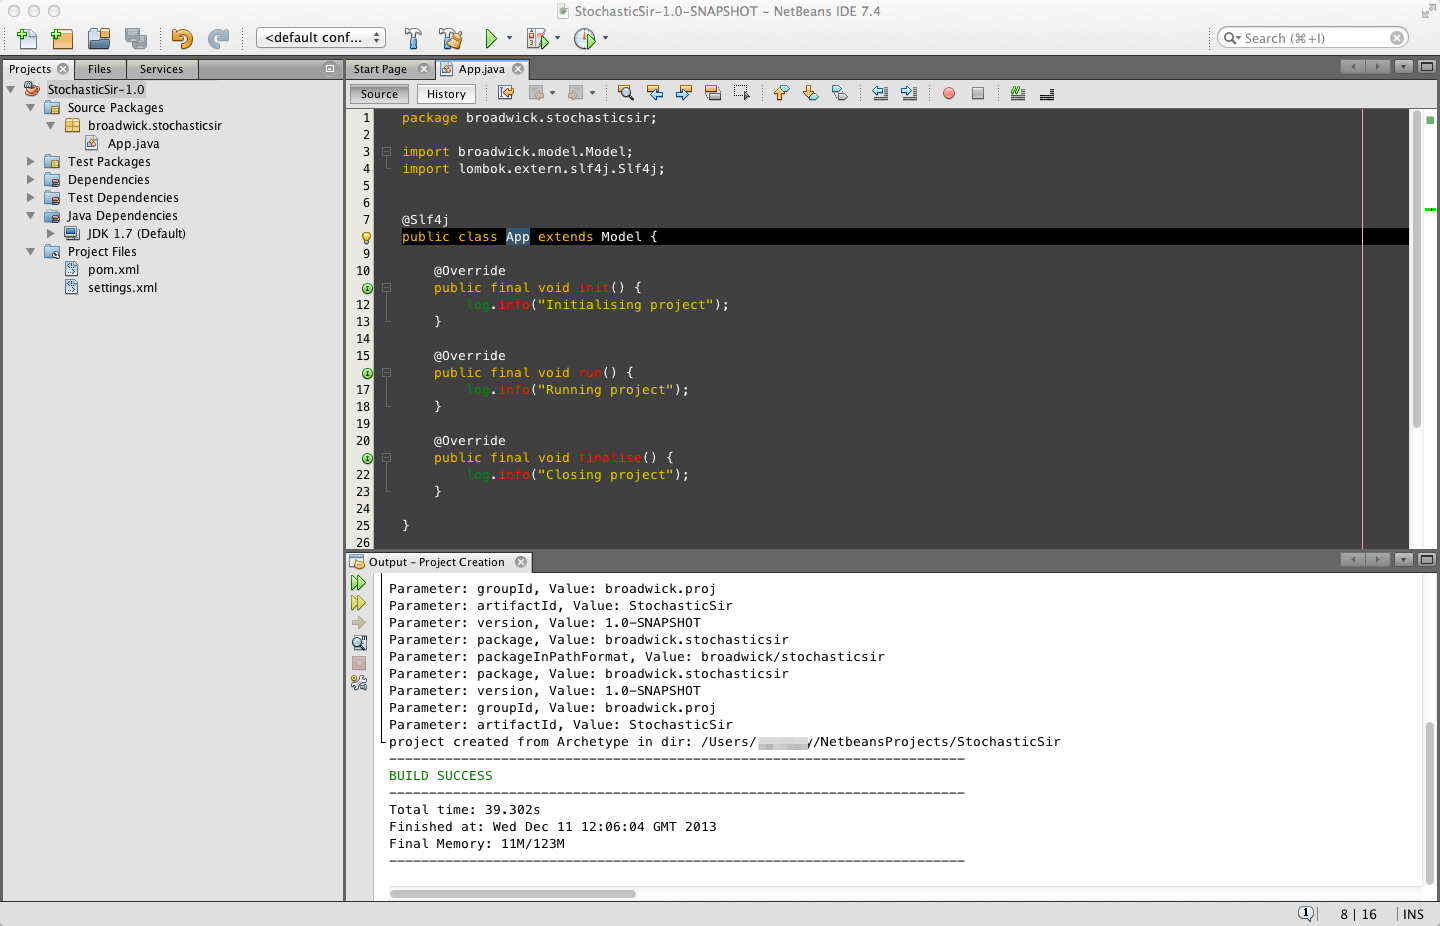
\includegraphics[width=12cm]{proj4.png}
\caption{The generated project}
\label{proj4}
\end{figure}

A number of minor changes are needed in the generated project.

Select the name of the class (``App”) and right-click and select Refactor->Rename; Change the name of the class to StochasticSIR.

In the Broadwick.sh file change the \$\{artifactId\} and \$\{version\} to the artifactId and version specified when the project was created (StochasticSIR and 1.0 respectively). This is a shell script for running your project on Unix based systems, you will need to make it executable.

In Broadwick.xml (the configuration file for the generated project) change the name of the <classname> element to reflect the package and class (broadwick.stochasticsir.StocasticSIR)

We can build the generated project by selecting Run->Build Project from the menu bar or clicking the 
\includegraphics[scale=0.22]{proj5.png} icon in the toolbar (see fig \ref{proj6} for some example output from this process). This will create a directory called target that contains, among other items, a jar file containing the compiled code and an executeable jar file ending in .one-jar.jar. The Broadwick.sh file is a shell script that will run the executable jar file on *NIX systems.

\begin{figure}[h!]
\centering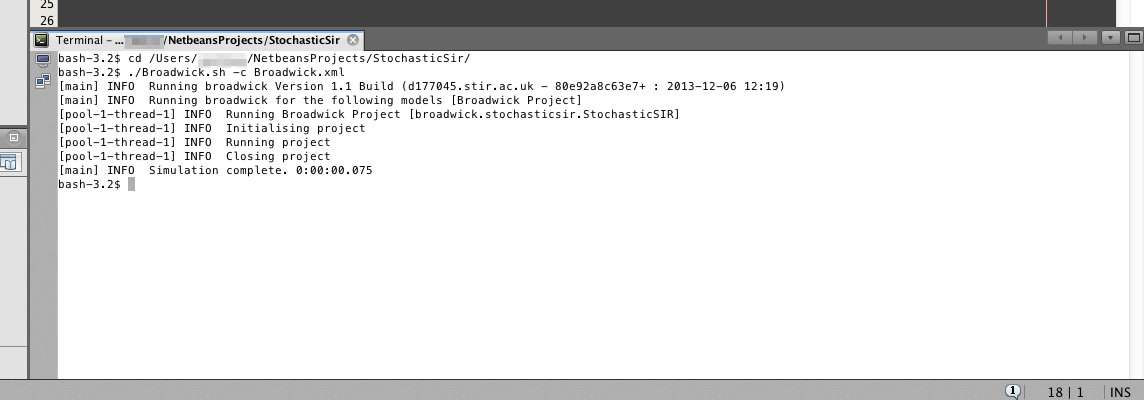
\includegraphics[width=12cm]{proj6.png}
\caption{Figure caption}
\label{proj6}
\end{figure}

When Broadwick starts it looks for all the models specified in the <model> elements in the projects configuration file. It creates objects for each <model> found using the default (empty) constructor for the class given in the <classname> element of the model (this is why no constructor is generated for the project).

For each project object created Broadwick will call the init(), run() and finalise() methods in turn. In our skeleton project we simply logged the fact that these methods were called. A simplified outline of how Broadwick initialises itself is shown in fig \ref{broadwicksummary}.

\begin{figure}[h!]
\centering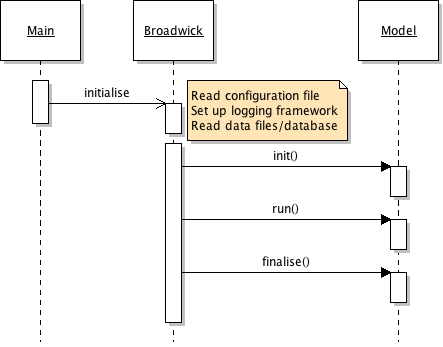
\includegraphics[width=8cm]{BroadwickSummary.png}
\caption{Schematic outline of the steps Broadwick performs on startup}
\label{broadwicksummary}
\end{figure}

A description of the configuration file is outlined in the next section.

\section{Configuration Files}\index{Configuration Files}

The configuration file MUST conform to the Broadwick.xsd specification that is supplied with the Broadwick source code. The configuration is contained within the <project> </project> tags and contains the following tags

\begin{tabulary}{1.0\textwidth}{llp{8cm}}
\toprule
<logs> & <console> & Contains <level> and <pattern> tags to define the level and structure of logging messages displayed on the console.\\
       & <files> & Contains <level> and <pattern> tags like the <console> log but also a <name> for the name of the file to contain the log messages and a boolean <overwrite> tag that lets Broadwick know if any existing file with that name should be overwritten.\\
<data> & <databases> & Contains the <name> tag to specify the location of the database.\\
       & <datafiles> & Contains the <DirectedMovementFile> <FullMovementFile> <BatchMovementFile> <PopulationFile> <LocationsFile> and <TestsFile> tags for the various file structures recognised by Broadwick. See the following tables in this section for a description of each.\\
<models> & <model> & Broadwick can run several models concurrently (though they will share the same logging and data configurations). \\
\bottomrule
\end{tabulary}

\vskip 1cm
Each model element contains the following:

\begin{tabulary}{0.3\linewidth}{l p{10cm}}
\toprule
<classname> & Exactly one classname element that is the fully qualified name of the java  class (that implements the broadwick.model.Model interface). This class MUST have a no argument constructor that Broadwick will use to create an instance through relection.\\
<priors> & The <priors> tag can contain as many elements as necessary, each prior contains an id attribute and optional <hint> and <initialVal> elements. The following priors are recognised by Broadwick\\
         & <uniformPrior> additionally contains <min> and <max> elements for uniformly distributed priors.\\
         & <gaussianprior> additionally contains <mean> and <deviation> tags for normally distributed priors.\\
         & <parameter> The parameters for the model can be encoded in this tag using the id and value attributes to name the parameters and give the parameter value. These can be accessed by the broadwick.model.Model getParameterAs[TYPE](id) method that retrieves the parameter with the given id and converts it the the required type.\\
\bottomrule
\end{tabulary}

Each datafile contains specific information on it’s layout, i.e. the columns in the file where the required data can be found. The structure of each recognised data file is outlined below.

DirectedMovementFile:

\begin{tabulary}{0.3\linewidth}{l p{9cm}}
\toprule
<name> & The name (including path from the configuration file) where the file can be found. \\
<alias> & An alias for the file. \\
<separator> & The character separating the columns in the datafile, e.g. `,' `<tab>'.\\
<idColumn> &  \\
<movementDateColumn> &  \\
<movementDirectionColumn> &  \\
<locationColumn> &  \\
<speciesColumn> &  \\
<dateFormat> &  The format the date is given in the data file, see below for details.\\
<customTags> & This optional field allows for optional information to be stored in the database. \\
\bottomrule
\end{tabulary}\\

FullMovementFile:

\begin{tabulary}{1.0\textwidth}{l p{9cm}}
\toprule
<name> & The name (including path from the configuration file) where the file can be found.\\
<alias> & An alias for the file.\\
<separator> & The character separating the columns in the datafile, e.g. `,' `<tab>'.\\
<idColumn> & \\
<departureDateColumn> & \\
<departureLocationIdColumn> & \\
<destinationDateColumn> & \\
<destinationLocationIdColumn> & \\
<marketIdColumn> & \\
<marketDateColumn> & \\
<speciesColumn> & \\
<dateFormat> & The format the date is given in the data file, see below for details.\\
<customTags> & This optional field allows for optional information to be stored in the database.\\
\bottomrule
\end{tabulary}\\

BatchMovementFile:

\begin{tabulary}{1.0\textwidth}{l p{9cm}}
\toprule
<name> & The name (including path from the configuration file) where the file can be found.\\
<alias> & An alias for the file.\\
<separator> & The character separating the columns in the datafile, e.g. `,' `<tab>'.\\
<batchSizeColumn> & \\
<departureDateColumn> & \\
<departureLocationIdColumn> & \\
<destinationDateColumn> & \\
<destinationLocationIdColumn> & \\
<marketIdColumn> & \\
<marketDateColumn> & \\
<speciesColumn> & \\
<dateFormat> & The format the date is given in the data file, see below for details.\\
<customTags> & This optional field allows for optional information to be stored in the database.\\
\bottomrule
\end{tabulary}\\

PopulationFile:

\begin{tabulary}{1.0\textwidth}{l p{9cm}}
\toprule
<name> & The name (including path from the configuration file) where the file can be found.\\
<alias> & An alias for the file.\\
<separator> & The character separating the columns in the datafile, e.g. `,' `<tab>'.\\
<lifehistory> & \\
<population> & \\
<speciesColumn> & \\
<dateFormat> & The format the date is given in the data file, see below for details.\\
<customTags> & This optional field allows for optional information to be stored in the database.\\
\bottomrule
\end{tabulary}

Lifehistory:

\begin{tabulary}{1.0\textwidth}{l p{9cm}}
\toprule
<name> & The name (including path from the configuration file) where the file can be found.\\
<alias> & An alias for the file.\\
<separator> & The character separating the columns in the datafile, e.g. `,' `<tab>'.\\
\bottomrule
\end{tabulary}

Population:

\begin{tabulary}{1.0\textwidth}{l p{9cm}}
\toprule
<name> & The name (including path from the configuration file) where the file can be found.\\
<alias> & An alias for the file.\\
<separator> & The character separating the columns in the datafile, e.g. `,' `<tab>'.\\
\bottomrule
\end{tabulary}

LocationFile:

\begin{tabulary}{1.0\textwidth}{l p{9cm}}
\toprule
<name> & The name (including path from the configuration file) where the file can be found.\\
<alias> & An alias for the file.\\
<separator> & The character separating the columns in the datafile, e.g. `,' `<tab>'.\\
<locationIdColumn> & The column in the file containing the id of the location.\\
<eastingColumn> & The column in the file containing the easting coordinate. Coordinates aren’t strictly adhered to in Broadwick so a simple y-coordinate is sufficient.\\
<northingColumn> & The column in the file containing the northing coordinate. Coordinates aren’t strictly adhered to in Broadwick so a simple x-coordinate is sufficient.\\
<dateFormat> & The format the date is given in the data file, see below for details.\\
<customTags> & This optional field allows for optional information to be stored in the database.\\
\bottomrule
\end{tabulary}

TestsFile:

\begin{tabulary}{1.0\textwidth}{l p{10cm}}
\toprule
<name> & The name (including path from the configuration file) where the file can be found.\\
<alias> & An alias for the file.\\
<separator> & The character separating the columns in the datafile, e.g. `,' `<tab>'.\\
<idColumn> & One of these is required, specifying whether the test is performed on an individual, group (e.g. herd) or location (must match the id in the Location file).\\
<groupIdColumn> & \\
<locationIdColumn> & \\
<testDateColumn> & \\
<postiveResultColumn> & \\
<negativeResultColumn> & \\
<dateFormat> & The format the date is given in the data file, see below for details.\\
<customTags> & This optional field allows for optional information to be stored in the database. \\
\bottomrule
\end{tabulary}

The date format specification follows the standard formatting for dates and times:

\begin{tabulary}{1.0\textwidth}{l p{10cm}}
\toprule
Symbol &Meaning              \\
 G     &era                  \\
 C     &century of era (>=0) \\
 Y     &year of era (>=0)    \\
 x     &year          \\
 w     &week of weekyear     \\
 e     &day of week          \\
 E     &day of week          \\
 y     &year                 \\
 D     &day of year          \\
 M     &month of year        \\
 d     &day of month         \\
 a     &halfday of day       \\
 K     &hour of halfday (0~11)      \\
 h     &clockhour of halfday (1~12) \\
 H     &hour of day (0~23)          \\
 k     &clockhour of day (1~24)     \\
 m     &minute of hour              \\
 s     &second of minute            \\
 S     &fraction of second          \\
 z     &time zone                   \\
 Z     &time zone offset/id         \\
 '     &escape for text             \\
 ''    &single quote                \\
\bottomrule
\end{tabulary}


A simplified configuration file is generated in the skeleton project. It contains configuration items for logging to console and to file for different logging levels (info, warning, error, debug, trace) and we can specify the pattern to apply to the log message.

\begin{sourcecode}
    \begin{verbatim}
<?xml version="1.0" encoding="UTF-8" standalone="yes"?>
<project>
    <logs>
        <console>
            <level>info</level>
            <pattern>[%thread] %-5level %msg %n</pattern>
        </console>
        <file>
            <name>broadwick.stochasticsir.log</name>
            <level>info</level>
            <pattern>[%thread] %-5level %msg %n</pattern>
            <overwrite>true</overwrite>
       </file>
    </logs>

    <models>
          <model id="Broadwick Project">
                 <classname>broadwick.stochsir.StochasticSIR</classname>
          </model>
    </models>
</project>
\end{verbatim}
\end{sourcecode}

Common logging patterns are:

\begin{tabulary}{1.0\textwidth}{l p{10cm}}
\toprule
\%C             & Outputs the fully-qualified class name of the caller issuing the logging request. \\
\%M  {\%method} & Outputs the method name where the logging request was issued. \\
\%L  {\%line}   & Outputs the line number from where the logging request was issued. \\
\%F  {\%file}   & Outputs the file name of the Java source file where the logging request was issued. This is not very fast and should be avoided. \\
\%d & Used to output the date of the logging event e.g. \%d{HH:mm:ss,SSS}  \\
\%m  (\%msg)    & Outputs the application-supplied message associated with the logging event. \\
\%t  (\%thread) & Outputs the name of the thread that generated the logging event. \\
\%n & Outputs the platform dependent line separator character or characters \\
\%r & Outputs the number of milliseconds elapsed since the start of the application until the creation of the logging event. \\
\%p  {\%level}  & Outputs the level of the logging event. \\
\bottomrule
\end{tabulary}


More details on logging patterns can be found at \url{http://logback.qos.ch/manual/layouts.html}.

The model section requires a <classname> giving the fully qualified class name and optional <priors> and <parameter> sections. 

\section{Extending the Model}\index{Extending the Model}

Our stochastic SIR model that we have created is a valid Broadwick model but does not perform any useful calculations. We will add some parameters to the configuration file and read (and log them) in the init() method.

Firstly, let us define beta and rho parameters for the susceptible->infectious rate and for the infectious->recovered rates respectively and parameters for the maximum time for which we will run the simulation and the name of a file in which we will save the time series data. To do this modify the configured model section by:

\begin{sourcecode}
\begin{verbatim}
<model id="Broadwick Project">
    <classname>broadwick.stochasticsir.StochasticSIR</classname>

    <parameter id="beta" value="0.2" />
    <parameter id="rho" value="0.3" />
    <parameter id="tMax" value="100" />
    <parameter id="outputFile" value="broadwick.stochasticSIR.dat" />
</model> 
\end{verbatim}
\end{sourcecode}

Now edit the init() method of the StochasticSir class as shown in fig \ref{proj7}.

\begin{figure}[h!]
\centering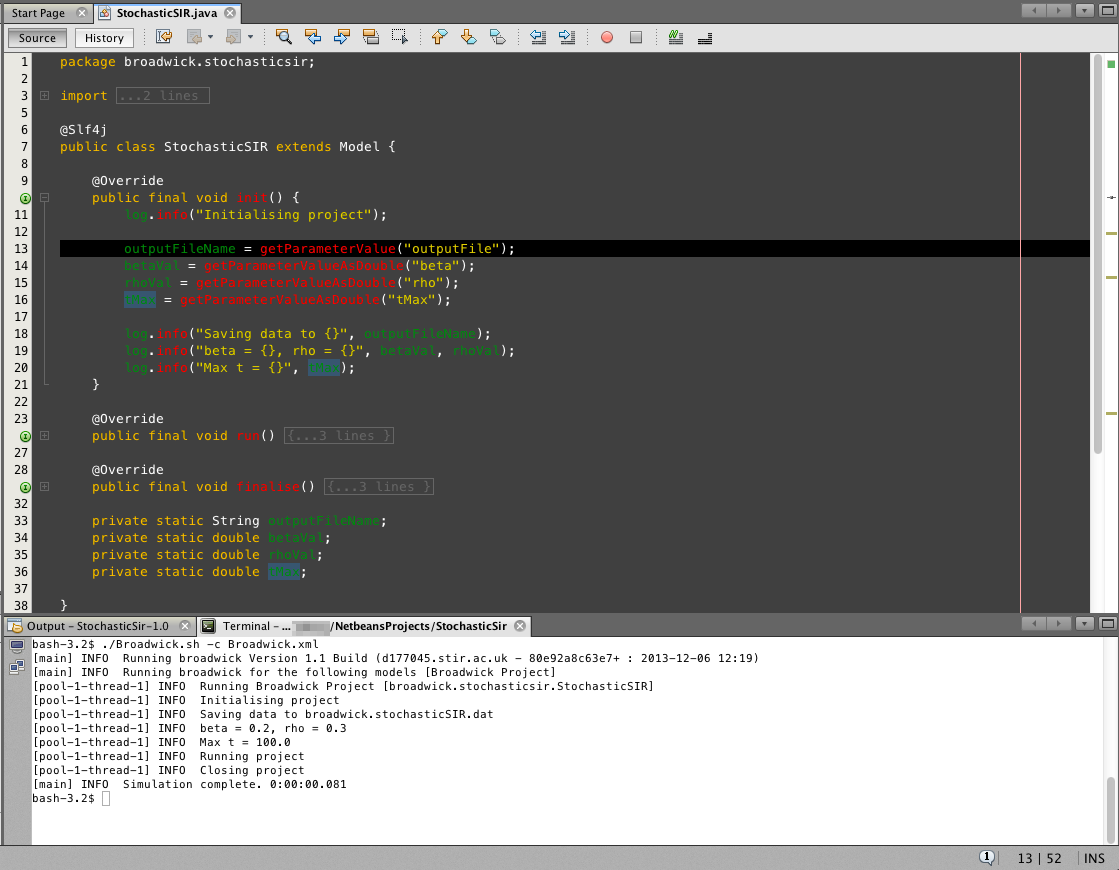
\includegraphics[width=12cm]{proj7.png}
\caption{Reading some parameters to our model}
\label{proj7}
\end{figure}

The `Model' class contains getParameterValue(String), getParameterValueAsDouble(String), getParameterValueAsInteger(String), getParameterValueAsBoolean(String) methods to extract parameters from the configuration file as strings (default), doubles, integers and booleans (if the parameter is written as ``true" or ``false").



\chapterimage{chapter_head_5.jpg} % Chapter heading image
\chapter{Calculation Packages}

Broadwick supports several simulation and fitting models. In this chapter we will give an outline of these methods and how they can be simulated (and combing) using the Broadwick framework. We will, for the most part, dispense with the theory referring the interested reader to relevent articles.




\section{Markov Chains}\index{Markov Chains}

A Markov chain is a random sequence of states where the current state depends solely on the previous state. In this sense, it is a ``memoryless'' process as the transition from one state to the next does not depend on the sequence of states that preceeded it.

A Markov Chain can be implemented in Broadwick using the MonteCarloStep and MarkovChain classes. The MonteCarloStep encapsulates the functionality of a state by maintaining a collection of the coordinates defining the state as a java.util.Map<String,Double> (i.e. the name and value of the state). A MarkovChain object is constructed using a MonteCarloStep object as an initial point and, optionally, a MarkovProposalFunction for generating the next step. The generateNextStep method uses the proposal function to generate the next step in the chain as the following code snippet demonstrates,

\begin{lstlisting}

final Map<String, Double> coordinates = new LinkedHashMap<>();
        {
            coordinates.put("x", 0.0);
            coordinates.put("y", 0.0);
        }
final MonteCarloStep initialStep = new MonteCarloStep(coordinates);

final MarkovChain mc = new MarkovChain(initialStep);
for (int i = 0; i < chainLength; i++) {
    final MonteCarloStep nextStep = mc.generateNextStep(mc.getCurrentStep());
    mc.setCurrentStep(nextStep);

    log.trace("{}", nextStep.toString());
}
\end{lstlisting}

By default, a MarkovNormalProposal object is used to generate the next step by sampling from a Normal distribution centered on the current coordinate and with a standard deviation of 1.


\section{Monte Carlo Simulation}\index{Monte Carlo Simulation}

\subsection{Markov Chain Monte Carlo}\index{Markov Chain Monte Carlo}

\section{Approximate Bayesian Computation (ABC)}\index{Approximate Bayesian Computation (ABC)}

\section{Ordinary Differential Equations (ODEs)}\index{Ordinary Differential Equations (ODEs)}





\chapterimage{chapter_head_6.jpg} % Chapter heading image
\chapter*{Appendix}

\section*{Maven as a Build Tool}\index{Maven, Using}

There is no requirement to use maven as a build tool but as Broadwick and it's examples are built using maven this section will give a brief outline of how maven is used to create a simple model.

Maven uses an xml file to describe the classes to be built as well as the dependencies, dynamically downloading required libraries as needed. It uses the 'convention over configuration' paradigm imposing the directory structure given in the table below. 



\begin{table}[h]
\centering
\begin{tabulary}{\textwidth}{l l}
\toprule
\textbf{Directory} & \textbf{Purpose}\\
\midrule
Project home & Contains the pom and all the subdirectories. \\
src/main/java & Contains the java source code for the project. \\
src/main/resources & Contains the xsd file for configuring the project. \\
src/test/java & Contains any [Junit or TestNG] test cases for the project. \\
src/test/resources & Contains resources necessary for testing. \\
\bottomrule
\end{tabulary}
%\caption*
{\\Maven's directory structure}
\end{table}

Maven's equivalent to a makefile or Ant's build.xml is a `project object model' which is stored in a pom.xml file. A good reference for the maven pom is http://maven.apache.org/pom.html.



%----------------------------------------------------------------------------------------
%	BIBLIOGRAPHY
%----------------------------------------------------------------------------------------

\chapterimage{chapter_head_bib.jpg} % Chapter heading image
\chapter*{Bibliography}
\addcontentsline{toc}{chapter}{\textcolor{ocre}{Bibliography}}
%\section*{Books}
%\addcontentsline{toc}{section}{Books}
%\printbibliography[heading=bibempty,type=book]
%\section*{Articles}
%\addcontentsline{toc}{section}{Articles}
\printbibliography[heading=bibempty,type=article]

%----------------------------------------------------------------------------------------
%	INDEX
%----------------------------------------------------------------------------------------

\cleardoublepage
\phantomsection
\setlength{\columnsep}{0.75cm}
\addcontentsline{toc}{chapter}{\textcolor{ocre}{Index}}
\printindex

%----------------------------------------------------------------------------------------

\end{document}
